\documentclass[a4paper,
fontsize=11pt,
%headings=small,
oneside,
numbers=noperiodatend,
parskip=half-,
bibliography=totoc,
final
]{scrartcl}

\usepackage[babel]{csquotes}
\usepackage{synttree}
\usepackage{graphicx}
\setkeys{Gin}{width=.4\textwidth} %default pics size

\graphicspath{{./plots/}}
\usepackage[ngerman]{babel}
\usepackage[T1]{fontenc}
%\usepackage{amsmath}
\usepackage[utf8x]{inputenc}
\usepackage [hyphens]{url}
\usepackage{booktabs} 
\usepackage[left=2.4cm,right=2.4cm,top=2.3cm,bottom=2cm,includeheadfoot]{geometry}
\usepackage[labelformat=empty]{caption} % option 'labelformat=empty]' to surpress adding "Abbildung 1:" or "Figure 1" before each caption / use parameter '\captionsetup{labelformat=empty}' instead to change this for just one caption
\usepackage{eurosym}
\usepackage{multirow}
\usepackage[ngerman]{varioref}
\setcapindent{1em}
\renewcommand{\labelitemi}{--}
\usepackage{paralist}
\usepackage{pdfpages}
\usepackage{lscape}
\usepackage{float}
\usepackage{acronym}
\usepackage{eurosym}
\usepackage{longtable,lscape}
\usepackage{mathpazo}
\usepackage[normalem]{ulem} %emphasize weiterhin kursiv
\usepackage[flushmargin,ragged]{footmisc} % left align footnote
\usepackage{ccicons} 
\setcapindent{0pt} % no indentation in captions

%%%% fancy LIBREAS URL color 
\usepackage{xcolor}
\definecolor{libreas}{RGB}{112,0,0}

\usepackage{listings}

\urlstyle{same}  % don't use monospace font for urls

\usepackage{xurl}

\usepackage[fleqn]{amsmath}

%adjust fontsize for part

\usepackage{sectsty}
\partfont{\large}

%Das BibTeX-Zeichen mit \BibTeX setzen:
\def\symbol#1{\char #1\relax}
\def\bsl{{\tt\symbol{'134}}}
\def\BibTeX{{\rm B\kern-.05em{\sc i\kern-.025em b}\kern-.08em
    T\kern-.1667em\lower.7ex\hbox{E}\kern-.125emX}}

\usepackage{fancyhdr}
\fancyhf{}
\pagestyle{fancyplain}
\fancyhead[R]{\thepage}

% make sure bookmarks are created eventough sections are not numbered!
% uncommend if sections are numbered (bookmarks created by default)
\makeatletter
\renewcommand\@seccntformat[1]{}
\makeatother

% typo setup
\clubpenalty = 10000
\widowpenalty = 10000
\displaywidowpenalty = 10000

\usepackage{hyperxmp}
\usepackage[colorlinks, linkcolor=black,citecolor=black, urlcolor=libreas,
breaklinks= true,bookmarks=true,bookmarksopen=true]{hyperref}
\usepackage{breakurl}

%meta
%meta

\fancyhead[L]{Chr. Erlinger \& J. Bemme\\ %author
LIBREAS. Library Ideas, 44 (2023). % journal, issue, volume.
%\href{https://doi.org/10.18452/27071}{\color{black}https://doi.org/10.18452/27071}
{}} % doi 
\fancyhead[R]{\thepage} %page number
\fancyfoot[L] {\ccLogo \ccAttribution\ \href{https://creativecommons.org/licenses/by/4.0/}{\color{black}Creative Commons BY 4.0}}  %licence
\fancyfoot[R] {ISSN: 1860-7950}

\title{\LARGE{Kamptaler Sakrallandschaften im Wikiversum} \vskip 1em \large{Edits mit Versionsgeschichte: Elementarteilchen offener Wissensproduktion am Beispiel eines Citizen Science-Projektes}}% title
\author{Christian Erlinger und Jens Bemme} % author

\setcounter{page}{1}

\hypersetup{%
      pdftitle={Kamptaler Sakrallandschaften im Wikiversum},
     pdfauthor={Christian Erlinger, Jens Bemme},
      pdfcopyright={CC BY 4.0 International},
      pdfsubject={LIBREAS. Library Ideas, 44 (2023).},
      pdfkeywords={Open access, Wikipedia, kollaboratives Schreiben, Sacherschließung},
      pdflicenseurl={https://creativecommons.org/licenses/by/4.0/},
      pdfurl={https://doi.org/},
      pdfdoi={10.18452/},
      pdflang={de},
      pdfmetalang={de}
     }



\date{}
\begin{document}

\maketitle
\thispagestyle{fancyplain} 

%abstracts
\begin{abstract}
\noindent
Die Autoren skizzieren, dass insbesondere lokales und regionales Wissen
mit Wikis entsteht und dauerhaft bleibt -- als Regionalia in globalen
offenen Linkzusammenhängen. ``Grass Root Open Access'' bedeutet nicht
nur, Publikationen auf selbst gezimmerte Art und Weise frei und unter
offener Lizenz zu publizieren (``I have published my pdf under a cc
license on my personal website''). ``Grass Root Open Science'' bedeutet
auch, den Inhalt, die Daten und Bilder -- das Wissen einer
publizistischen Arbeit an sich frei, offen und reproduzierbar zu
veröffentlichen. Am Beispiel der ``Wikifizierung'' einer gedruckten,
heimatkundlichen Buchpublikation wird gezeigt, wie mit
Graswurzelstrategien im Wikiversums Open Science entsteht.

Wir skizzieren einen solchen Prozess als `linked open': Methoden und
Effekte regionaler Datenpflege als demokratisierende Praxis mittels
Citizen Science, mit Blick auf Technologien und Gemeinschaften.
Potentiell beeinflussen wir mit offenen, wiki-basierten und damit
dezentralen Wissenssystemen die Kalkulation und Rentabilität
öffentlicher und quasi-öffentlicher Investitionen in Bildungsressourcen,
Informationsinfrastrukturen, Forschung und Entwicklung.
\end{abstract}

%body
\hypertarget{einleitung}{%
\section{Einleitung}\label{einleitung}}

Das gängige Verständnis von Open Access umfasst den kosten- und
möglichst barrierefreien elektronischen Zugang zu (wissenschaftlicher)
Literatur (OA 2002) oder weiter gefasst die Zugänglichkeit zu Wissen (OA
2003). Der 2003 ausgerufene Übergang zum \enquote{Open-Access-Pa\-ra\-dig\-ma
für elektronische Publikationen} (OA 2003) ist heute von der
Realisierung weit entfernt und maximal eines von Bibliotheken und
Forschungsförderung getriebenes Tätigkeitsfeld. Der Blick in das
Programm der Open-Access-Tage 2023 genügt, um zu sehen, wie bürokratisch
Open Access ist: Kosten-Monitoring, Evaluation und Management der
Transformation -- all das nimmt viel Raum und Zeit ein und kostet
Ressourcen.\footnote{Programm der Open-Access-Tage 2023
  \url{https://open-access-tage.de/open-access-tage-2023-berlin}, Stand
  28.10.2023}

Das Fundament der Bürokratie rund um Open Access und Open Science ist
die wissenschaftliche Produktion. Versuchen wir im Bibliotheksbereich
Publikation, Dokumentation und Vernetzung von wissenschaftlichen
Erkenntnissen -- ganz gleich ob aus institutioneller oder
bürger:in\-nen-wissenschaftlicher Produktion -- losgelöst von
verlegerischen Ansprüchen mit einfachen technischen Hilfsmitteln dem
simplen Grundsatz der kosten- und barrierefreien elektronischen
Zugänglichkeit folgend zu realisieren, so sind die technischen
Hilfsmittel die Gefäße oder Wurzeln, in denen die Forschung wachsen
kann: \enquote{Grassroot Open Science}. Damit begeben wir uns auf den
Boden wissenschaftlicher Kommunikation, wo die publizierten Inhalte von
heute, der Humus sind, auf dem neue Erkenntnisse morgen entstehen
können.

\hypertarget{open-public-humanities-regionalgeschichte-und-offene-wissenschaft}{%
\section{Open Public Humanities -- Regionalgeschichte und Offene
Wissenschaft}\label{open-public-humanities-regionalgeschichte-und-offene-wissenschaft}}

Citizen Science und Open Access wird in der Gemeinsamkeit bislang,
abgesehen von Ausnahmen (Munke 2019), kaum diskutiert. Das mag
einerseits daran liegen, dass Citizen Science oft als ein partizipativer
Methodenkasten institutionalisierter Wissenschaft missverstanden wird,
deren Ergebnisse dann wieder in das \enquote{klassische}
Publikationssystem einfließen. Oder weil es in kaum einer Bibliothek
Aufgabe ist, Bürger:innen in ihren \enquote{privaten Forschungen}
Publikationsunterstützung zu geben. Doch genau darin liegt ein lohnendes
Tätigkeitsfeld, das helfen kann, auch in Bibliotheken ein Methodenset
aufzubauen, das für jede andere Anwendung einer offenen Wissenschaft
genutzt werden kann.

Regional- und Heimatgeschichte ist eines der typischen Forschungsgebiete
für ein Feld mit hohem Einsatz von Bürger:innen. Als Hypothese lässt
sich formulieren, dass gerade in diesem Feld die gedruckte Publikation,
ob als Monographie in kleinster Auflage, im Selbstverlag oder als
Beitrag in regionalen Blättern, einen hohen Stellenwert genießt. Viele
Arbeiten sind stark \enquote{datengetrieben}, wenn darin beispielsweise
Inventare von regionalhistorisch bedeutenden Personen, Bauwerken oder
Ereignissen umfassend recherchiert und mittels Archivmaterialien,
Bilddokumenten und anderen Quellenmaterialien zusammengestellt werden.
Ziel einer \enquote{Grassroot-Open-Science-Transformation} in diesem
Bereich muss daher nicht die bloße kostenfreie, elektronische
Publikation sein, sondern vielmehr das offene Verfügbarmachen der
grundlegenden Inhalte und Daten im Sinne von \enquote{open public
humanities} (Erlinger 2022b). Ein idealer Ort, um heterogene Daten in
strukturierter Form, neben Bildern und Textmaterialien dauerhaft und
offen online zugänglich sowie auch nachnutzbar zu machen, ist das
\emph{Wikiversum} (Kloppenburg \& Schwarzkopf 2016).

\hypertarget{vom-buch-zum-datensatz-im-wikiversum}{%
\section{\texorpdfstring{Vom Buch zum Datensatz im
\emph{Wikiversum}}{Vom Buch zum Datensatz im Wikiversum}}\label{vom-buch-zum-datensatz-im-wikiversum}}

Im Herbst 2020 wurde auf der Website des \enquote{Zeitbrücke-Museums} in
Gars am Kamp (Niederösterreich)\footnote{Website des Zeitbrücke Museums
  Gars am Kamp (Niederösterreich) \url{https://www.zeitbruecke.at/},
  Stand: 28.10.2023} der Hinweis veröffentlicht, dass der damalige
Leiter des Museums, der Maler und Lehrer Anton Ehrenberger,
beabsichtigt, eine umfassende Dokumentation aller sakralen
Kleindenkmäler in der Umgebung des Ortes zu verfassen und in Form eines
Bildbandes im Eigenverlag zu veröffentlichen (Ehrenberger 2022).
Kleindenkmalforschung ist ein Paradebeispiel von datengestützter,
regionalwissenschaftlicher Forschungsarbeit mit einem hohen Grad quasi
vollständiger Dokumentation eines Kulturgutbestandes zu einem bestimmten
Zeitpunkt. Diese Ankündigung war der Anstoß dafür, dass ein Autor dieses
Beitrags den Kleindenkmalforscher kontaktierte, um gemeinsam einen
möglichst umfassenden Open Science-Ansatz auszuprobieren:

\begin{itemize}
\item
  Das (selbst erstellte) Bildmaterial wird unter der Lizenz CC BY 4.0
  auf Wikimedia Commons hochgeladen.
\item
  Jedes beschriebene Objekt erhält ein eigenständiges Wikidata-Item und
  wird mit den im Buch veröffentlichten Informationen weitestgehend
  beschrieben. Diese Daten sind unter CC 0 lizenziert.
\end{itemize}

Das Ergebnis der Zusammenarbeit ist ein öffentlich verfügbarer
Datensatz, der jederzeit wiederverwendet werden kann und dem durch die
grundlegenden Eigenschaften der Software MediaWiki (die zum Beispiel für
die Wikipedia genutzt wird) wesentliche Elemente einer offenen
Wissenschaft automatisch innewohnen:

\begin{itemize}
\item
  Jeder Edit ist Teil einer Versionsgeschichte. Veränderungen am
  Datensatz sind offen zugänglich und können überprüft werden.
\item
  Fehler können korrigiert werden. Fortlaufende, zukünftige
  Veränderungen am Forschungsobjekt können eingepflegt werden.
\item
  Diskussionsseiten erlauben das Besprechen der eingearbeiteten Inhalte.
  Fehler und Zweifel können diskutiert werden.
\end{itemize}

Die Übertragung der Daten aus dem Buch war eine zeitintensive und in
erster Linie manuelle Tätigkeit. Gleichzeitig war dies eine besondere
Art des gründlichen Korrekturlesens und wurde somit zu einer auch
inhaltlichen Unterstützung in der Forschungsarbeit selbst. Das
Übertragen der schriftlichen Informationen in strukturierte Daten in die
Datenbank Wikidata (mit der unter anderem Daten für die Wikipedia
bereitgestellt werden), förderte Ungereimtheiten zu Tage und half Fehler
zu erkennen.

In der nachfolgenden Tabelle ist beispielhaft angegeben, welche
Eigenschaften in Wikidata für ein Objekt, im vorliegenden Fall das
\enquote{Obenaus-Marterl}\footnote{Obenaus-Marterl, Wikidata-Item
  Q38093425 \url{https://www.wikidata.org/wiki/Q38093425}, Stand:
  28.10.2023} gewählt wurden und welche Bedeutung diese tragen
(Entnommen aus Erlinger 2022a).

\documentclass[a4paper,
fontsize=11pt,
%headings=small,
oneside,
numbers=noperiodatend,
parskip=half-,
bibliography=totoc,
final
]{scrartcl}

\usepackage[babel]{csquotes}
\usepackage{synttree}
\usepackage{graphicx}
\setkeys{Gin}{width=.95\textwidth} %default pics size

\graphicspath{{./plots/}}
\usepackage[ngerman]{babel}
\usepackage[T1]{fontenc}
%\usepackage{amsmath}
\usepackage[utf8x]{inputenc}
\usepackage [hyphens]{url}
\usepackage{booktabs} 
\usepackage[left=2.4cm,right=2.4cm,top=2.3cm,bottom=2cm,includeheadfoot]{geometry}
\usepackage{eurosym}
\usepackage{multirow}
\usepackage[ngerman]{varioref}
\setcapindent{1em}
\renewcommand{\labelitemi}{--}
\usepackage{paralist}
\usepackage{pdfpages}
\usepackage{lscape}
\usepackage{float}
\usepackage{acronym}
\usepackage{eurosym}
\usepackage{longtable,lscape}
\usepackage{mathpazo}
\usepackage[normalem]{ulem} %emphasize weiterhin kursiv
\usepackage[flushmargin,ragged]{footmisc} % left align footnote
\usepackage{ccicons} 
\setcapindent{0pt} % no indentation in captions

%%%% fancy LIBREAS URL color 
\usepackage{xcolor}
\definecolor{libreas}{RGB}{112,0,0}

\usepackage{listings}
\usepackage{tabularx}

\urlstyle{same}  % don't use monospace font for urls

\usepackage[fleqn]{amsmath}

%adjust fontsize for part

\usepackage{sectsty}
\partfont{\large}

%Das BibTeX-Zeichen mit \BibTeX setzen:
\def\symbol#1{\char #1\relax}
\def\bsl{{\tt\symbol{'134}}}
\def\BibTeX{{\rm B\kern-.05em{\sc i\kern-.025em b}\kern-.08em
    T\kern-.1667em\lower.7ex\hbox{E}\kern-.125emX}}

\usepackage{fancyhdr}
\fancyhf{}
\pagestyle{fancyplain}
\fancyhead[R]{\thepage}

% make sure bookmarks are created eventough sections are not numbered!
% uncommend if sections are numbered (bookmarks created by default)
\makeatletter
\renewcommand\@seccntformat[1]{}
\makeatother

% typo setup
\clubpenalty = 10000
\widowpenalty = 10000
\displaywidowpenalty = 10000

\usepackage{hyperxmp}
\usepackage[colorlinks, linkcolor=black,citecolor=black, urlcolor=libreas,
breaklinks= true,bookmarks=true,bookmarksopen=true]{hyperref}
\usepackage{breakurl}

%meta
%meta

\fancyhead[L]{N. Haupka, N. Jahn, A. Hobert\\ %author
LIBREAS. Library Ideas, 41 (2022). % journal, issue, volume.
%\href{https://doi.org/10.18452/xxx}{\color{black}https://doi.org/10.18452/xxx}
{}} % doi 
\fancyhead[R]{\thepage} %page number
\fancyfoot[L] {\ccLogo \ccAttribution\ \href{https://creativecommons.org/licenses/by/4.0/}{\color{black}Creative Commons BY 4.0}}  %licence
\fancyfoot[R] {ISSN: 1860-7950}

\title{\LARGE{Praxisbericht Big Scholarly Data an der SUB Göttingen}}% title
\author{Nick Haupka, Najko Jahn, Anne Hobert} % author

\setcounter{page}{1}

\hypersetup{%
      pdftitle={Praxisbericht Big Scholarly Data an der SUB Göttingen},
      pdfauthor={Nick Haupka, Najko Jahn, Anne Hobert},
      pdfcopyright={CC BY 4.0 International},
      pdfsubject={LIBREAS. Library Ideas, 41 (2022)},
      pdfkeywords={Big Scholarly Data, Bibliometrie,Open Access Transformation,Hybrides Open Access},
      pdflicenseurl={https://creativecommons.org/licenses/by/4.0/},
      pdfcontacturl={http://libreas.eu},
      baseurl={},
      pdflang={de},
      pdfmetalang={de}
     }
   



\date{}
\begin{document}

\maketitle
\thispagestyle{fancyplain} 

%abstracts
\begin{abstract}
\noindent
Der Beitrag stellt den Einsatz des kommerziellen
Cloud-Computing-Dienstes Google BigQuery für die Arbeit mit großen
offenen Datensätzen über wissenschaftliche Veröffentlichungen an der
Nidersächsischen Staats- und Universitätsbibliothek Göttingen (SUB
Göttingen) vor, insbesondere bezogen auf den Datenbestand, die
Prozessierung und die Zugriffsmöglichkeiten. Als beispielhafter Use Case
werden überregionale Open-Access-Transformationsverträgen in Deutschland
bezogen auf ihren Open-Access-Anteil analysiert.
\end{abstract}

%body
\hypertarget{motivation}{%
\section{Motivation}\label{motivation}}

An der Niedersächsischen Staats- und Universitätsbibliothek Göttingen
(SUB Göttingen) führen wir als Data-Analysis-Team für Wissenschaftliche
Information regelmäßig Analysen von Daten über wissenschaftliche
Publikationen durch. Dabei untersuchen wir Fragestellungen im
Zusammenhang bibliometrischer Forschungsprojekte, wollen aber auch
datengestützte strategische Entscheidungen an unserer Universität und
darüber hinaus ermöglichen.

Unser Augenmerk liegt auf frei verfügbaren großen Datensätze über
wissenschaftliche Informationsprozesse, sogenannte Big Scholarly Data.
Deren Offenheit ermöglicht es uns, ohne hohe Investitionskosten etwa für
die Lizenzierung einer Datenquelle Analysen durchzuführen. Offene Daten
erhöhen zudem die Transparenz unserer Analysen, da wir sowohl Daten als
auch Analysecode gemeinsam mit unseren Berichten offen verfügbar machen
können. Zudem sind wir ein kleines Team und daher auf die Zusammenarbeit
mit Kolleg*innen anderer Einrichtungen angewiesen, mit denen wir
jederzeit auf den gleichen Datenpool zugreifen können, was mit offenen
Daten prinzipiell möglich ist.

Bei unserer Arbeit mit Big Scholarly Data hat sich schnell
herausgestellt, dass wir einen verteilten und hochperformanten Zugriff
benötigen. Große Datensätze über wissenschaftliche Publikationen werden
hauptsächlich als (unbearbeitete, nicht vollständig strukturierte)
Datendumps bereitgestellt, deren lokale Prozessierung sehr aufwendig und
wegen fehlender Rechenkapazitäten nur bedingt möglich ist. Wichtig war
uns zudem, auch ohne ausgeprägte Kenntnisse der Datenbank- und
Serveradministration, gemeinsam Datenanalysen durchführen zu können. Aus
diesem Grunde verwenden wir die Cloud-basierte Datenbankumgebung Google
BigQuery, ein serverloses Data Warehouse für die hochperformante Analyse
großer Datenbestände.\footnote{\url{https://cloud.google.com/bigquery?hl=de}}

Begonnen haben wir mit Google BigQuery im Jahr 2019, und zwar mit dem
Download und der Prozessierung der Datensnapshots des
Open-Access-Discovery-Services Unpaywall\footnote{\url{https://unpaywall.org/}}.
Die Snapshots haben wir im Rahmen des BMBF-Forschungsprojekts
OAUNI\footnote{\url{https://www.wihoforschung.de/wihoforschung/de/bmbf-projektfoerderung/foerderlinien/quantitative-wissenschaftsforschung/oauni/oauni_node.html}}
aufbereitet, um Unpaywall dahingehend zu analysieren, welche
Informationen zum Open-Access-Status wissenschaftlicher Publikationen in
der Datenquelle enthalten sind.\footnote{Siehe zum Beispiel Jahn et
  al.~(2021) und Hobert et al.~(2021).} Mit der Zeit konnten wir unsere
Routinen zur Datenaufbereitung verfeinern und unser Portfolio durch
Hinzunahme zusätzlicher Datenquellen wie Crossref oder OpenAlex
erweitern.

Im Beitrag beschreiben wir, wie wir mit Google BigQuery arbeiten,
insbesondere den Datenbestand, die Prozessierung und die
Zugriffsmöglichkeiten. Zur Illustration geben wir einen kurzen Einblick
in die aktuelle Entwicklung von Dashboards zur Wirksamkeit von
Transformationsverträgen in Deutschland, die wir im Rahmen eines
DFG-Projekts zur Kostentransparenz des Lizenzmodells entwickeln.

\hypertarget{verfuxfcgbare-daten-innerhalb-der-google-bigquery-instanz}{%
\section{Verfügbare Daten innerhalb der Google
BigQuery-Instanz}\label{verfuxfcgbare-daten-innerhalb-der-google-bigquery-instanz}}

Unsere BigQuery-Instanz umfasst im Wesentlichen drei Datenquellen, die
wir pflegen und kuratieren: Unpaywall, Crossref und OpenAlex. Zu jeder
dieser Quellen existieren Schnittstellen, die es erlauben, einen
Snapshot der jeweiligen Datenquelle herunterzuladen. Die Snapshots
prozessieren wir entsprechend unserer datenanalytischen Anforderungen.
So liegt der Fokus unserer Arbeit häufig auf Veröffentlichungen in
wissenschaftlichen Journalen, weshalb wir oftmals keine kompletten
Snapshots in unsere Instanz überführen, sondern eine Teilmenge, die sich
auf Zeitschriftenartikel bezieht.

Unsere BigQuery Data Warehouse ist dabei so aufgebaut, dass wir zu jeder
Quelle sowohl einen aktuellen (\emph{current}) als auch historische
(\emph{historical}) Snapshots anbieten. Historische Snapshots werden in
regelmäßigen Abständen (zum Beispiel jährlich) gesichert, sodass die
Entwicklung und Qualität einer Datenbank über einen zeitlichen Verlauf
beurteilt werden kann. Diese Snapshots verwenden wir auch für unsere
wissenschaftlichen Publikationen, da sie im Gegensatz zum regelmäßig
aktualisierten Datensatz (\emph{current}), niemals überschrieben werden.
Dadurch gewährleisten wir die Reproduzierbarkeit unserer Analysen. Der
jeweils aktuelle Snapshot (\emph{current}) benutzen wir in unseren
Dashboards und anderen Analysen, die einen möglichst aktuellen Bezug
erfordern und hauptsächlich die Bibliothekspraxis adressieren.

Die von uns bereitgestellten Snapshots können sich, wie angedeutet, von
den Snapshots der Datenbankanbieter leicht unterscheiden. So filtern wir
gezielt nach Zeitschriftenartikeln, entfernen Datenfelder und grenzen
das Publikationsvolumen auf bestimmte Jahre ein. Unsere bereitgestellten
Unpaywall-Snapshots enthalten beispielsweise nur Zeitschriftenartikel ab
2008, unsere Crossref-Tabellen hingegen Zeitschriftenartikel ab 2013.
Lediglich die OpenAlex-Snapshots befinden sich unverändert auf unserer
BigQuery-Instanz, da wir derzeit noch nicht einschätzen können, welche
Informationen in OpenAlex wir zukünftig auswerten möchten.

\hypertarget{prozessierung}{%
\subsection{Prozessierung}\label{prozessierung}}

Für jede der genannten Datenquellen haben wir eine Prozedur entwickelt,
die die Überführung eines Snapshots in BigQuery ermöglicht. Die dabei
angewandten Schritte lassen sich in Download,
Prozessierung/Transformation, Upload und Erstellung einer Tabelle in
BigQuery unterteilen.

Im ersten Schritt wird ein Big-Scholarly-Data-Snapshot auf Server der
Gesellschaft für wissenschaftliche Datenverarbeitung mbH Göttingen
(GWDG), die als Rechenzentrum der Universität Göttingen fungiert,
heruntergeladen. Im zweiten Schritt verwenden wir Skripte, die es
ermöglichen, die Datenbestände zu filtern, Datenfelder zu entfernen und
Zeittransformationen durchzuführen. Hiermit soll erreicht werden, dass
sich die Größe des Snapshots reduziert, wodurch wir
Cloud-Computing-Kosten sparen. Da die Snapshots meist sehr umfangreich
sind und mehrere hundert Gigabyte umfassen können, verwenden wir für die
Datentransformation das High Performance Cluster (HPC) der GWDG. Dieser
Service erlaubt es uns, durch die Bereitstellung leistungsstarker
Server, mit großen Datenmengen zu arbeiten. Je nach Konfiguration und
Datenbank kann die Transformation auf dem HPC mehrere Stunden dauern.
Das Resultat wird daraufhin in ein \enquote*{Google Bucket} geladen. Von
da aus kann eine Tabelle in BigQuery erstellt werden. Tabelle 1 zeigt
die von uns bereitgestellten Datenbanken sowie die angewendeten
Prozeduren.

Tabelle 1: Informationen zu den bereitgestellten Snapshots
\begin{longtable}[]{@{}
  >{\raggedright\arraybackslash}p{(\columnwidth - 4\tabcolsep) * \real{0.15}}
  >{\raggedright\arraybackslash}p{(\columnwidth - 4\tabcolsep) * \real{0.42}}
  >{\raggedright\arraybackslash}p{(\columnwidth - 4\tabcolsep) * \real{0.42}}@{}}
\toprule
Datenbank & Download & Prozedur \\
\midrule
\endhead
Unpaywall & Unpaywall-Snapshots werden in regelmäigen Abständen auf
einem Amazon S3 Cloud Storage angeboten. Die Snapshots sind in der Regel
zwischen 16 und 30 Gigabyte groß. Der Download ist kostenlos. Ein
Account wird nicht benötigt. & Bei der Prozessierung des Snapshots
verwenden wir das Command-Line-Tool jq
(\url{https://stedolan.github.io/jq/}) und das Programm parallel
(\url{https://www.gnu.org/software/parallel/}). Das von uns verwendete
Skript wird auf Github angeboten
(\url{https://github.com/naustica/unpaywall_bq}). \\
Crossref & Crossref veröffentlicht jeden Monat einen Datenbanksnapshot
als Teil der kostenpflichtigen Metadata-Plus-Mitgliedschaft
(\url{https://www.crossref.org/services/metadata-retrieval/metadata-plus/}).
Die Snapshots können dabei im XML- oder JSON-Format heruntergeladen
werden. Die Snapshots enthalten viele kleine Dateien, die in einem
tar-Archiv zusammengefasst werden. Die Snapshots sind zwischen 100 und
160 Gigabyte groß. & Unser verwendetes Skript basiert auf Arbeiten des
Academic Observatory
(\url{https://github.com/The-Academic-Observatory/academic-observatory-workflows}).
Wir haben dieses Skript leicht verändert, sodass es auf unseren Servern
läuft. Das von uns verwendete Skript wird auf Github angeboten
(\url{https://github.com/naustica/crossref_bq}). \\
OpenAlex & Der OpenAlex-Snapshot wird in fünf Entitäten unterteilt.
Diese sind Works, Authors, Venues, Institutions und Concepts. Jede
dieser Entitäten kann einzeln aber auch zusammen mit den anderen
Entitäten heruntergeladen werden. Der Download ist kostenlos. Der
komplette Snapshot umfasst mehrere hundert Gigabyte. & Der
OpenAlex-Snapshot ist so aufgebaut, dass er theoretisch ohne weitere
Bearbeitung in Google BigQuery geladen werden kann. Dennoch verwenden
wir auch hierfür ein Skript, welches uns ermöglicht Datenfelder zu
bearbeiten und zu filtern. Das von uns verwendete Skript wird auf Github
angeboten (\url{https://github.com/naustica/openalex}). \\
\bottomrule
\end{longtable}


\hypertarget{zugriffsoptionen}{%
\subsection{Zugriffsoptionen}\label{zugriffsoptionen}}

Es existieren verschiedene Zugriffsmöglichkeiten auf BigQuery. Die
Google Cloud console bietet eine webbasierte grafische
Benutzeroberfläche, mit der sämtliche Ressourcen verwaltet und
SQL-Anfragen ausgeführt werden können. Es ist möglich, SQL-Anfragen
projektbezogen zu teilen. Zudem lässt sich auf BigQuery mit den uns
vertrauten Programmiersprachen R und Python zugreifen.

Die Autorisierung und Authentifizierung erfolgt wie etwa bei GoogleDocs
über Google-Accounts. Ein umfassendes Rechtemanagement ermöglicht es
uns, externe Kolleg*innen einzuladen und ihnen angepasste Rollen für den
Datenzugriff einzuräumen. Es lassen sich zudem Zugriffstoken erstellen,
etwa wenn Abfragen durch einen Continuous Integration und Continuous
Delivery (CI/CD) Service wie GitHub Actions automatisch ausgeführt
werden sollen.

Das folgende Beispiel illustriert den Zugriff auf unser BigQuery
Datawarehouse mit R und dem Client bigrquery (Wickham \& Bryan, 2021).
Nach erfolgter Authentifizierung fragen wir den aktuellen
Crossref-Snapshot mittels SQL nach den Top 10 Verlagen mit Artikeln
unter einer Creative-Commons-Lizenz ab. Die Ergebnistabelle kann
entweder innerhalb der BigQuery-Cloud-Umgebung gespeichert oder lokal
heruntergeladen werden.

\begin{verbatim}
library(bigrquery)
 
# Authentification
my_con <- bigrquery::bq_auth()
# SQL example
 
# Top 10 publishers by the number of articles with Creative Commons
# license in Crossref
my_query <- "SELECT
  publisher,
  COUNT(DISTINCT(DOI)) AS n
FROM
  `subugoe-collaborative.cr_instant.snapshot`,
  UNNEST(license) AS license
WHERE
  REGEXP_CONTAINS(license.URL, 'creativecommons')
GROUP BY
  publisher
ORDER BY
  n DESC
LIMIT
  10"
# Call Big Query
tb <- bigrquery::bq_project_query("subugoe-collaborative",
                              query = my_query)
# Download results
bigrquery::bq_table_download(tb)
#> # A tibble: 10 × 2
#>  publisher                                      n
#>  <chr>                                         <int>
#>  1 Elsevier BV                                 775742
#>  2 Springer Science and Business Media LLC     745306
#>  3 MDPI AG                                     731206
#>  4 IOP Publishing                              342991
#>  5 Public Library of Science (PLoS)            241008
#>  6 Wiley                                       232884
#>  7 Hindawi Limited                             215611
#>  8 Frontiers Media SA                          212607
#>  9 Informa UK Limited                          166956
#> 10 Walter de Gruyter GmbH                      106683
\end{verbatim}

\hypertarget{organisatorische-aspekte}{%
\subsection{Organisatorische Aspekte}\label{organisatorische-aspekte}}

Kommerzielle Cloud-Services wie Google Cloud rechnen ihre Kosten bezogen
auf die Nutzung ab. Bei Google BigQuery gibt es zwei Kostenarten:
Speicher- und Abfragevolumen. Beliefen sich die monatlichen Kosten zu
Beginn zunächst auf 2€, so liegen sie seit der Integration von OpenAlex
und Crossref zwischen 20 und 30€.

Die Rechnungen lassen sich im Rahmen einer Auslagenerstattung
einreichen, was aus Sicht der Verwaltung nur eine Übergangslösung ist.
Mittlerweile schließen Rechenzentrumsverbünde wie GÉANT
Rahmenvereinbarungen mit Cloud-Computing-Anbietern an. Daher arbeiten
wir derzeit im Austausch mit unserem federführenden Rechenzentrum, der
GWDG, daran, dass wir als Pilot im Zuge einer solchen
Infrastructure-as-a-Service-Vereinbarung auf einen zentralen
Google-Cloud-Account wechseln. Dadurch könnte die Rechnungslegung
künftig zentral erfolgen.

\hypertarget{use-case-hybrides-open-access-im-rahmen-von-transformationsvertruxe4gen-in-deutschland}{%
\section{Use Case: Hybrides Open Access im Rahmen von
Transformationsverträgen in
Deutschland}\label{use-case-hybrides-open-access-im-rahmen-von-transformationsvertruxe4gen-in-deutschland}}

Als Anwendungsbeispiel stellen wir das R-Paket hoaddata\footnote{\url{https://subugoe.github.io/hoaddata/}}
vor, das derzeit im Rahmen des DFG-Projekts Hybrid Open Access
Dashboards (HOAD) entwickelt wird. Der Fokus des Projekts, welches als
Fonds- und Workflowprojekt der Ausschreibung \enquote{Open Access
Transformationsverträge} gefördert wird, liegt auf datenanalytischen
Hilfestellungen zur Transparenz des Erwerbungsmodells. Insbesondere die
Bemessung des Open-Access-Anteils wissenschaftlicher Artikel bezogen auf
ein Verlagsportfolio mit hybriden Journalen stellt nach wie vor ein
diesbezügliches Desiderat dar (Jahn et al.~2022).

Aufgabe des R-Pakets hoaddata ist die automatische und kontinuierliche
Abfrage und Transformation von Daten über konsortiale
Transformationsverträge in Deutschland mittels unseres BigQuery Data
Warehouse. Ein R-Paket ist eine standardisierte und reproduzierbare
Dokumentation-, Test- und Programmierumgebung, die nicht nur Funktionen,
sondern auch Daten umfasst. hoaddata bildet als R-Datenpaket die
Grundlage für die Dashboardentwicklungen im Projekt, kann aber auch für
andere Analysen mit R genutzt werden.

hoaddata stützt sich auf Pollack et al.~(2022), um eine Liste von
Zeitschriften zu erhalten, die unter diesen Vereinbarungen stehen und
die vom deutschen Open-Access-Monitor (OAM) verwendet wird. Bevor diese
in hoaddata überführt wurden, haben wir die Zeitschriftenangaben in
einer einzigen Datei zusammengefasst und diese mit ISSN-Varianten
einschließlich ISSN-L angereichert. Da es keinen direkten Datenaustausch
zwischen ISSN-Agenturen und Crossref zu geben scheint\footnote{\url{https://community.crossref.org/t/parallel-titles-for-a-given-issn/2183}},
haben wir außerdem die OAM-Zeitschriftenliste mit der
Crossref-Titelliste abgeglichen, um Crossref-Zeitschriftentitel
eindeutig zu identifizieren.

Auf Grundlage der Zeitschriftenliste ermittelten wir bei Crossref das
Artikelvolumen je Zeitschrift und Jahr unter Verwendung unseres BigQuery
Data Warehouse. Zur Bestimmung des Open-Access-Status werteten wir die
von Crossref bereitgestellten Creative-Commons-Lizenzinformationen aus,
welche bezogen auf die verschiedenen Lizenzversionen normalisiert
wurden.

Da die Länderzugehörigkeit ein wichtiger Datenpunkt für nationale
Transformationsverträge ist, nutzen wir OpenAlex, um den
Ländermarktanteil je Zeitschrift und Verlagsportfolio zu ermitteln. Da
OpenAlex unseres Wissens nach keine Informationen über
Korrespondenzautor*innen und deren Affiliationen liefert, haben wir
stattdessen die Zugehörigkeit der Erstautor*innen herangezogen. Ein*e
Erstautor*in wird oft als Lead Author betrachtet, welche*r in der Regel
den größten Teil der im Artikel dargestellten Forschungsarbeit geleistet
hat, wobei die Rolle von Autor*innen je nach Fachgebiet variieren
kann.\footnote{\url{https://en.wikipedia.org/wiki/Lead_author}} In den
Fällen, in denen OpenAlex keine Länderzugehörigkeit verzeichnet,
extrahierten wir die Ländernamen aus dem Adressfeld mit Hilfe regulärer
Ausdrücke.

Das R-Paket hoaddata wird automatisch mit GitHub Actions erstellt. Jedes
Merge-Ereignis im Hauptzweig löst eine Datenaktualisierung auf Grundlage
unseres BigQuery Data Warehouse aus. Datenaktualiserungen werden dadurch
kontinuierlich in das Paket aufgenommen und mit Git nachverfolgt. Dies
macht es einfach, verschiedene Versionen der in hoaddata enthaltenen
Daten zu aktualisieren und zu reproduzieren.

Mitte Mai 2022 umfasst hoaddata 5.573 hybride Journale, die in zwanzig
Transformationsverträgen enthalten sind. Für den Zeitraum ab 2017
enthält hoaddata Daten über das Open-Access-Publikationsaufkommen von
5.562 hybriden Journalen. Die Diskrepanz zur
Ausgangszeitschriftentitelliste erklärt sich dadurch, dass Verlage wie
Springer Nature weiterhin hybride Journale gründen, die noch keine
Artikel veröffentlicht haben. Ein Beispiel ist das Journal Digital
Society, welches von Luciano Floridi herausgeben wird und Teil der
DEAL-Vereinbarung ist.\footnote{\url{https://www.springer.com/journal/44206}}
Neben den zeitschriftenbezogenen Informationen über das
(Open-Access)-Publikationsaufkommen und das Affiliationsprofil
beinhaltet hoaddata Metadaten der Open-Access-Artikel in hybriden
Journalen auf Artikelebene. Insgesamt verzeichnet hoaddata 348.978
Artikel unter einer Creative-Commons-Lizenz.

\begin{figure}
\centering
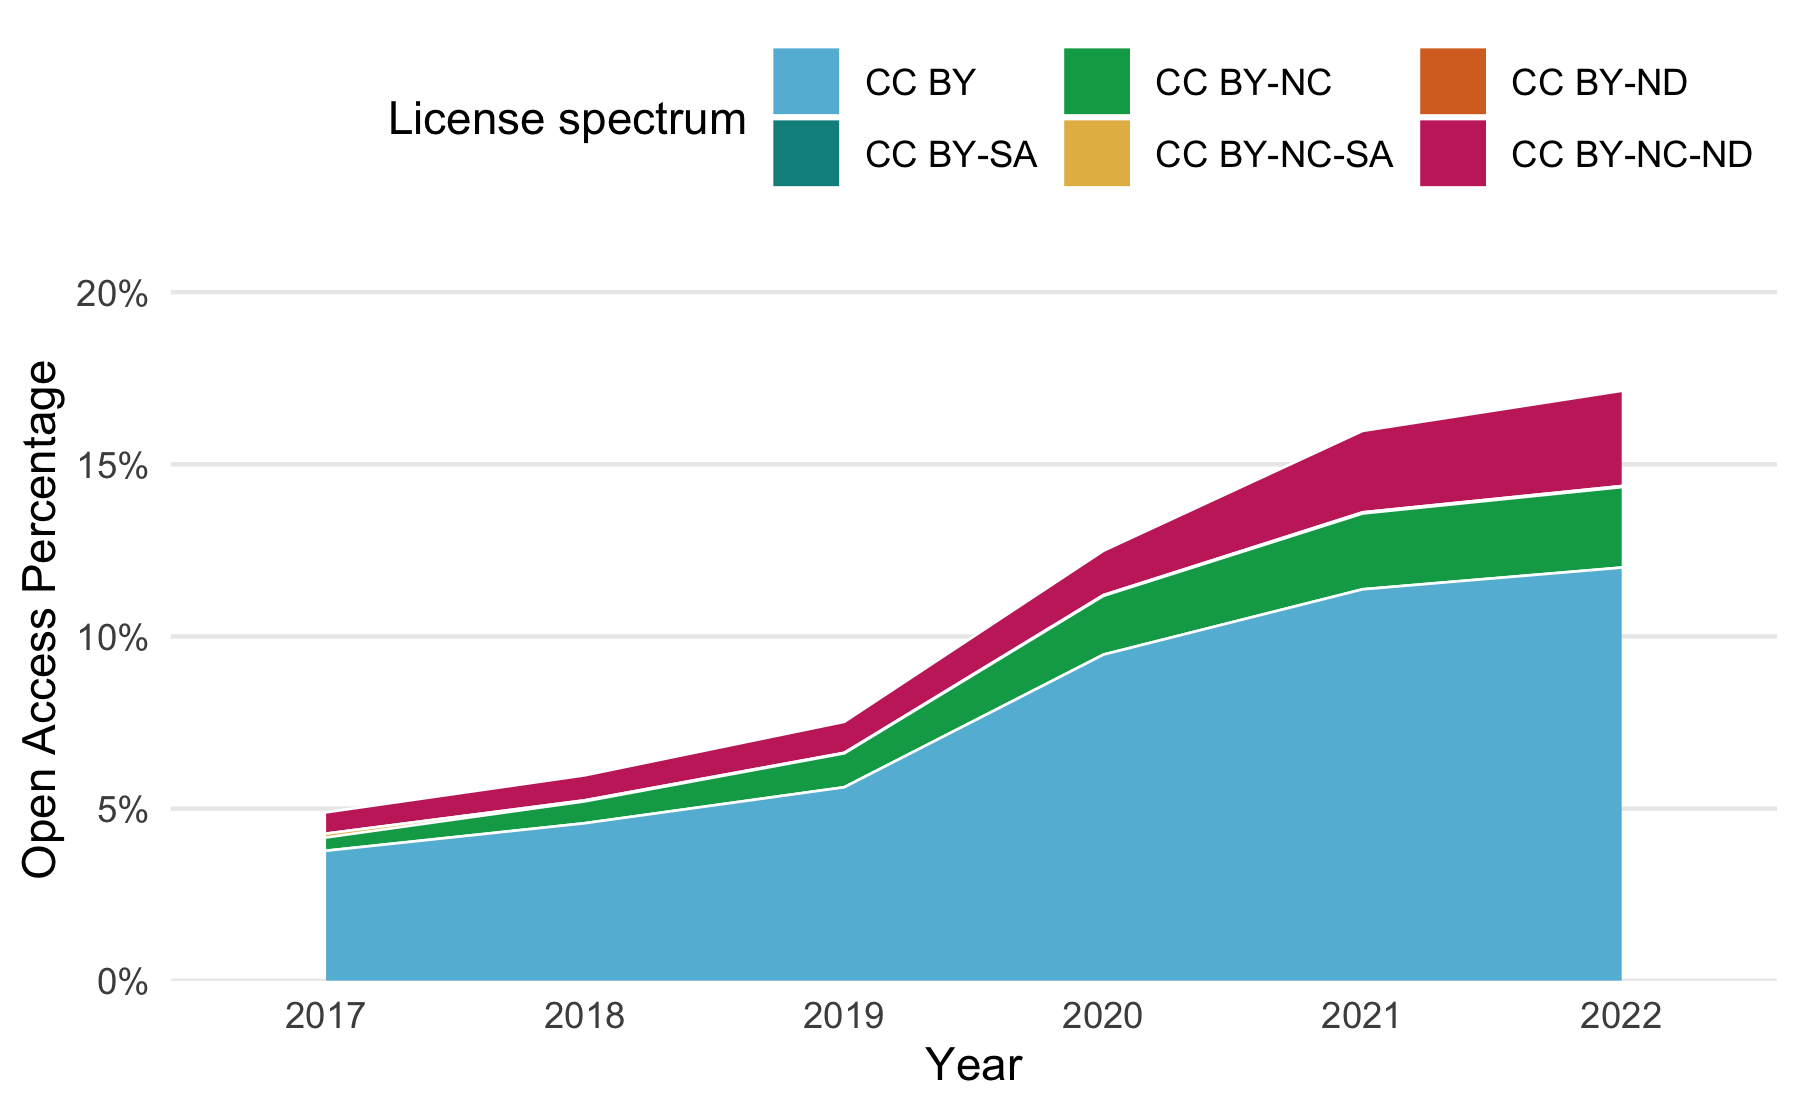
\includegraphics{fig/fig_1.png}
\caption{Abbildung 1: Relative Entwicklung des globalen
Open-Access-Anteils in hybriden Journalen, welche durch konsortiale
Transformationsverträge in Deutschland mit kommerziellen Verlagen
abgedeckt sind. Datenquellen: Pollack et al.~(2022) und Crossref
(Datenstand März 2022).}
\end{figure}

Abbildung 1 zeigt die prozentuale Entwicklung des Open-Access-Anteils in
hybriden Journalen, welche durch konsortiale Transformationsverträge in
Deutschland abgedeckt sind. Es zeigt sich, dass trotz der gestiegenen
Bedeutung von Open-Access-Transformationsverträgen nur jeder sechste
Artikel in diesen Journalen Open Access publiziert wurde. Ein Großteil
der Artikel wurde unter der Variante CC BY veröffentlicht, welche im
Vergleich zu den anderen Varianten eine umfassende Nachnutzung
ermöglicht.

\begin{figure}
\centering
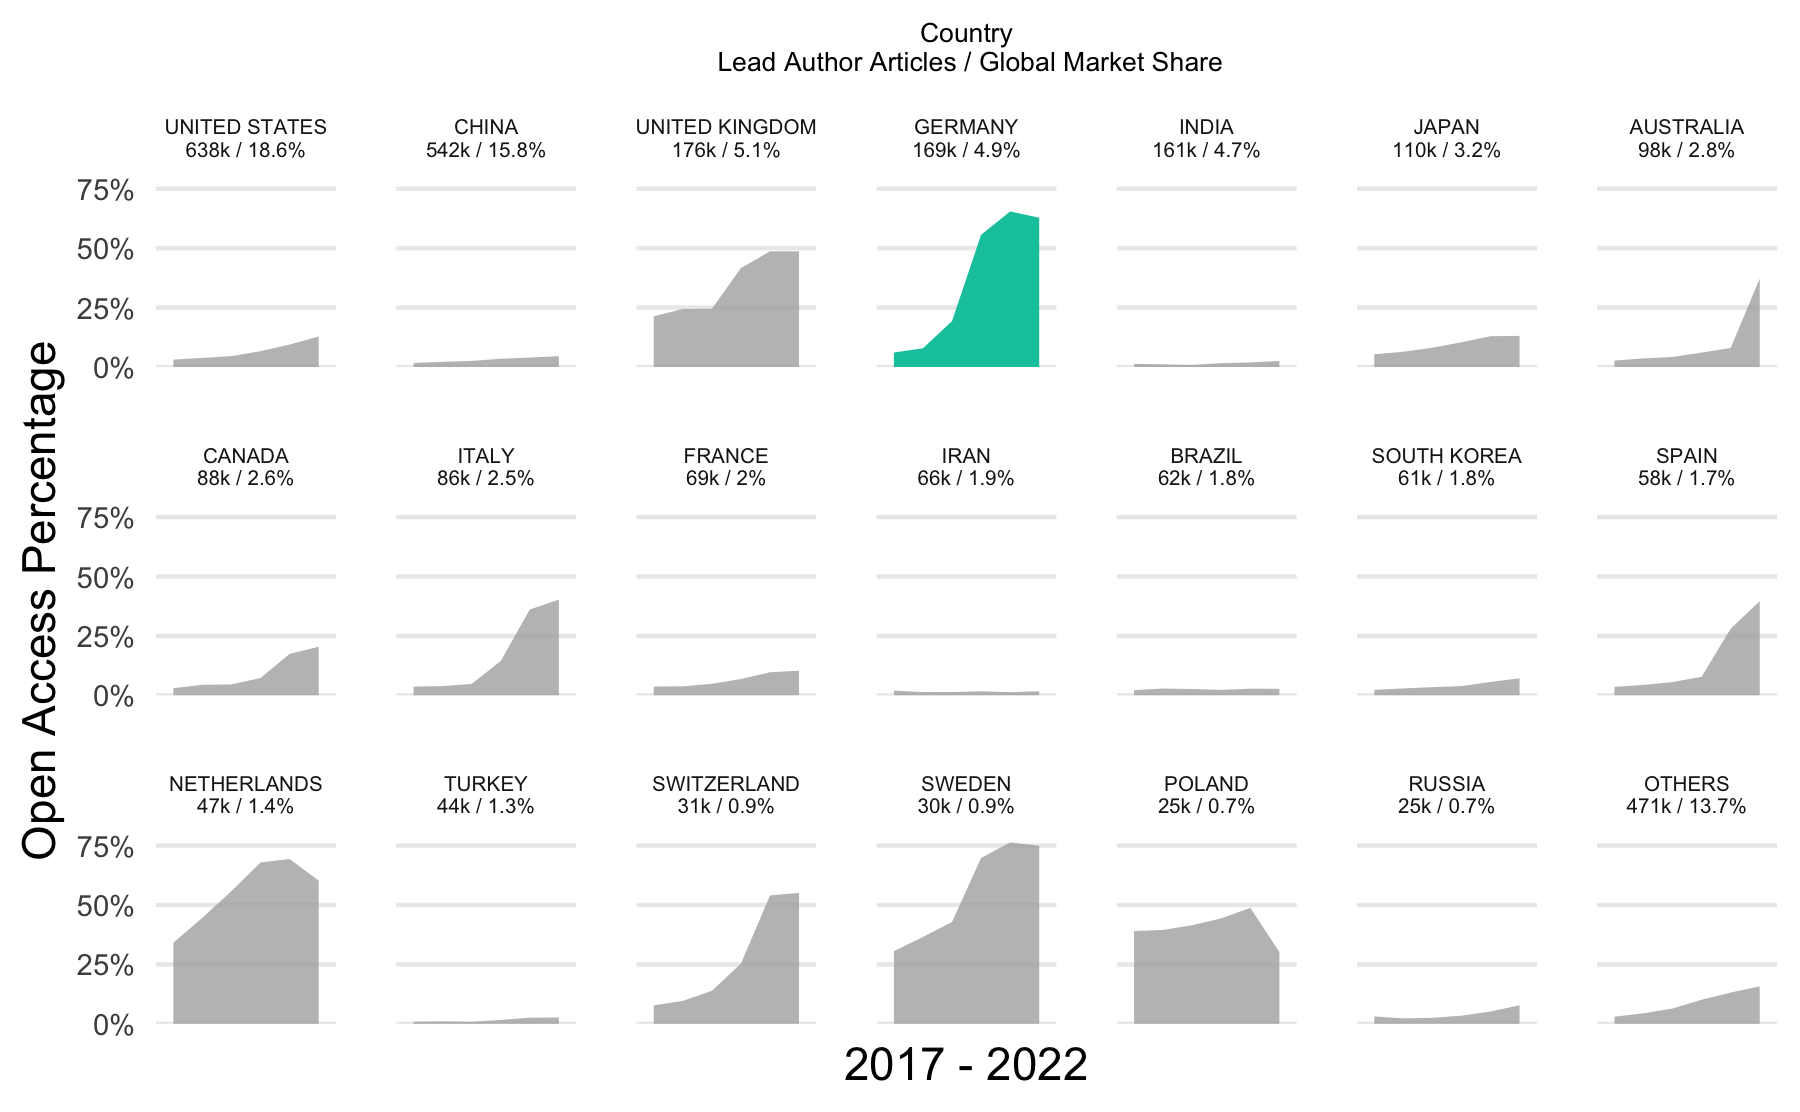
\includegraphics{fig/fig_2.png}
\caption{Abbildung 2: Relative Entwicklung des Open-Access-Anteils in
hybriden Journalen, welche durch konsortiale Transformationsverträge in
Deutschland mit kommerziellen Verlagen abgedeckt sind je Land.
Abgebildet sind die 20 publikationsstärksten Länder. Länderspezifische
Zwischenüberschriften beinhalten die Gesamtzahl der Publikationen im
Zeitraum sowie deren prozentualer Anteil am untersuchten
Gesamtpublikationsvolumen. Datenquellen: Pollack et al.~(2022), Crossref
und OpenAlex.*}
\end{figure}

Abbildung 2 zeigt den Open-Access-Anteil für die zwanzig
publikationsstärksten Länder gemessen an der Adresse der Erstautor*innen
(\emph{lead author}) und liefert damit ein Indiz, warum Open Access im
hybriden Portfolio der konsortialen Transformationsverträge in
Deutschland weiterhin eine Ausnahme darstellt. Der OA-Anteil in den
publikationsstarken Ländern USA und China ist aufgrund fehlender
nationaler Open-Access-Vereinbarungen weitaus geringer im Vergleich zu
den europäischen Ländern Deutschland, Großbritannien, den Niederlanden
oder Schweden. Die Abbildung zeigt zudem den geringen Open-Access-Anteil
in den asiatischen Ländern Japan und Südkorea oder bei Middle Income
Countries (MICs) wie Indien, Brasilien, Türkei oder Iran. Interessant
ist, dass der Open-Access-Anteil deutscher Artikel im Jahr 2021 trotz
umfangreicher Transformationsverträge bei unter 70\,\% lag.

\hypertarget{diskussion-und-ausblick}{%
\section{Diskussion und Ausblick}\label{diskussion-und-ausblick}}

Ein Cloud-basiertes Hosting von frei verfügbaren Big Scholarly Data
ermöglicht uns unabhängig von Data-Analytics-Angeboten
wissenschaftlicher Verlage umfassende Analysen der Wandlungsprozesse des
wissenschaftlichen Publizierens. Damit machen wir uns nicht nur vom
Datentracking der Anbieter unabhängig (Lauer, 2022), sondern können
zugleich alternative und offene Data-Analytics-Angebote entwickeln.

Nichtsdestotrotz spielen Fragen der Datenabdeckung und -qualität offener
Daten über wissenschaftliche Veröffentlichungen eine wesentliche Rolle.
Wir adressieren dieses Spannungsfeld zum einen über die Beteiligung an
Abdeckungsanalysen im Kontext unserer Mitgliedschaft im Kompetenzzentrum
Bibliometrie\footnote{\url{https://www.bibliometrie.info/}}. Zum anderen
sehen wir im Sinne der ESAC Guidelines\footnote{\url{https://esac-initiative.org/about/transformative-agreements/guidelines-for-transformative-agreements/}}
Wissenschaftliche Bibliotheken in der Verantwortung, auf umfangreiche
und qualitätsbewusste Metadaten bei Verlagen (nicht nur) im Kontext von
Open-Access-Transformationsverträgen hinzuwirken (Geschuhn und Stone,
2017, Voigt, 2020). Zur Unterstützung der Metadatenüberprüfung stellen
wir mit metacheck\footnote{\url{https://subugoe.github.io/metacheck/}}
ein frei verfügbares Werkzeug bereit.

Mittlerweile nutzen wir unser Data Warehouse, das auf BigQuery basiert,
umfangreich in unseren Projekten und für wissenschaftliche
Publikationsvorhaben. Der größte Pluspunkt ist die hohe
Leistungsfähigkeit von BigQuery. Dass komplexe Abfragen von Datensätzen,
deren Dateigrößen im Bereich einer zwei- bis dreistelligen Anzahl
Gigabytes liegen, innerhalb von Sekunden Ergebnisse liefern, ist
großartig und sehr komfortabel. Etwas Vergleichbares könnten wir mit
einer selbst gehosteten Datenbank nicht erreichen. Zudem können wir
Kolleg*innen aus externen Einrichtungen Zugriff auf die Datenbank geben,
etwa im erweiterten Kontext der ESAC Data Analytics Group\footnote{\url{https://esac-initiative.org/about/data-analytics/esac-data-working-group}}
oder des Kompetenzzentrums Bibliometrie. Dank der anstehenden Migration
in einen institutionellen Account unserer Universität durch eine
Rahmenvereinbarung verbessern wir zudem die organisatorische Einbindung
der dienstlichen Nutzung des Cloud-basierten Data Warehouse.

International ist zu beobachten, dass BigQuery in vergleichbaren
Zusammenhängen genutzt wird. Insbesondere die australische Curtin Open
Knowledge Initiative (COKI)\footnote{\url{https://openknowledge.community/}}
mit ihren frei verfügbaren Workflows zur Integration von Big Scholarly
Data in BigQuery ist für uns vorbildlich.\footnote{\url{https://academic-observatory-workflows.readthedocs.io/en/latest/}}
Es stellt sich daher zukünftig die Frage nach Kooperation und Synergien
bezüglich der Bereitstellung und Analyse offener Daten über
wissenschaftliche Veröffentlichungen mittels BigQuery.

\hypertarget{literatur}{%
\section{Literatur}\label{literatur}}

Geschuhn, Kai und Graham Stone. \enquote{It's the Workflows, Stupid!
What Is Required to Make \enquote*{Offsetting} Work for the Open Access
Transition}. \emph{Insights the UKSG Journal} 30, Nr. 3 (8. November
2017): 103--14. \url{https://doi.org/10.1629/uksg.391}.

Hobert, Anne, Najko Jahn, Philipp Mayr, Birgit Schmidt und Niels
Taubert. \enquote{Open Access Uptake in Germany 2010--2018: Adoption in
a Diverse Research Landscape}. \emph{Scientometrics} 126, Nr. 12 (2021):
9751--77. \url{https://doi.org/10.1007/s11192-021-04002-0}.

Jahn, Najko, Maximilian Held, Henrieke Walter, Nick Haupka und Kristine
Hillenkötter. \enquote{HOAD: Data Analytics Für Mehr Transparenz Bei
Open-Access-Transformationsverträgen}. \emph{ABI Technik} 42, Nr. 1
(2022): 64--69. \url{https://doi.org/10.1515/abitech-2022-0007}.

Jahn, Najko, Anne Hobert und Nick Haupka. \enquote{Entwicklung und
Typologie des Datendiensts Unpaywall}. \emph{Bibliothek Forschung und
Praxis} 45, Nr. 2 (2021): 293--303.
\url{https://doi.org/10.1515/bfp-2020-0115}.

Lauer, Gerhard. \enquote{Datentracking in den Wissenschaften}.
\emph{o-bib. Das offene Bibliotheksjournal} 9, Nr. 1 (2022).
\url{https://doi.org/10.5282/O-BIB/5796}.

Pollack, Philipp, Barbara Lindstrot, Irene Barbers und Franziska
Stanzel. \enquote{Open Access Monitor: Zeitschriftenlisten}. Jülich
DATA, 2022. \url{https://doi.org/10.26165/JUELICH-DATA/VTQXLM}.

Voigt, Michaela. \enquote{DEAL Open-Access-Option optimal nutzen -- ein
Bibliothekspraxisbericht}, LIBREAS.Library Ideas, 38 (2020).
\url{https://libreas.eu/ausgabe38/voigt/}.

Wickham, Hadley und Jennifer Bryan. \emph{bigrquery: An Interface to
Google's \enquote{BigQuery} \enquote{API}} (R package version 1.4.0),
2021.
\href{https://cran.r-project.org/package=bigrquery}{https://CRAN.R-project.org/package=bigrquery}.

%autor
\begin{center}\rule{0.5\linewidth}{0.5pt}\end{center}

\textbf{Nick Haupka}, \textbf{Najko Jahn} und \textbf{Dr.~Anne Hobert}
arbeiten an der Niedersächsischen Staats- und Universitätsbibliothek
(SUB) in der Gruppe Wissen als Gemeingut und sind dort mit Datenanalysen
im Kontext Wissenschaftlicher Information betraut. Mehr Infos:
\url{https://subugoe.github.io/scholcomm_analytics/about.html}

\end{document}


Die ausgewählten Datenfelder der Tabelle sind exemplarisch jene Werte,
die für das beschriebene Kleindenkmal bekannt sind. Die Flexibilität von
Wikidata erlaubt aber die Erfassung weiterer detaillierter
Informationen, beziehungsweise, die Daten können jederzeit um weitere
\enquote{Datenfelder} ergänzt sowie auf Normdaten verlinkt werden:

\begin{itemize}
\item
  Verlinkung und damit Referenzierung einer Vielzahl externer
  Datenbanken oder Websites wie zum Beispiel marterl.at
  (\url{https://www.marterl.at/}) oder die Gemeinsame Normdatei der
  Deutschen Nationalbibliothek (GND).
\item
  Es können signifikante Ereignisse (Renovierung, Weihe) hinzugefügt und
  detailliert werden.
\item
  Das Denkmal kann noch näher beschrieben werden: Baustil oder Epoche,
  Größe, verwendetes Material et cetera.
\item
  Erfassung von Details wie Abbildungen oder Inschriften.
\end{itemize}

Gerade die Verlinkungen der beschriebenen Objekte mit gegebenenfalls der
GND, mit der Datenbank des österreichischen Bundesdenkmalamtes oder
anderen Quellen, war eine Tätigkeit, die klassisch bibliothekarisch
motiviert war und die in der Buchpublikation befindlichen Inhalte
darüber hinaus inhaltlich kontextualisierte. Umgekehrt wurden im
gedruckten Buch sehr viele historische Quellenangaben zu den einzelnen
Dokumenten notiert -- bei vielen dieser Quellen handelt es sich
ebenfalls um graue Literatur. Abgesehen von der österreichischen
Kunsttopographie, die Open Access verfügbar ist,\footnote{Digitalisat
  der Österreichischen Kunsttopographie (1889), TUGraz DIGITAL Library,
  \url{https://diglib.tugraz.at/oesterreichische-kunsttopographie-1889},
  Stand: 28.10.2023} wurden noch keine weiteren Quellenangaben für das
vorgestellte Projekt in Wikidata systematisch erfasst.

Die Erfassung dieser Daten im \emph{Wikiversum} lädt unmittelbar dazu
ein, solche Informationen mit anderen Daten und Objekten zu verbinden,
die im Buch selbst nicht beschrieben sind, zum Beispiel aus
Platzgründen. Dazu zählen neben der erwähnten Normdaten-Verlinkung auch
Verbindungen zu Wikipedia-Artikeln oder die Vernetzung mit
Bildmaterialien in Wikimedia Commons (und dazu die Erzeugung von
Kategorien in Commons zur Sammlung von mehreren Mediendateien des
gleichen Denkmals).

Da die Daten nicht nur frei verfügbar und nutzbar, sondern auch
beständig weiter editierbar sind - \enquote{it's a wiki!} - wurde
bereits während der Drucklegung des Buches die Forschung fortgeführt. So
konnten Renovierungen von Denkmälern erfasst werden oder auch Fehler,
die trotz mehrfacher Korrekturläufe erst spät entdeckt wurden, zumindest
im offenen Datensatz behoben werden. Dem Datenmodell von Wikidata sei
Dank, brauchen solche Fehler nicht einfach überschrieben werden, sondern
können als \enquote{deprecated} mit der entsprechenden Quellenangabe
erfasst werden. Dies erlaubt ein digitales Erratum zur Publikation zu
erstellen.\footnote{Wikidata SPARQL-Query \enquote{Errata der
  Publikation \enquote*{Kamptaler Sakrallandschaften}},
  \url{https://w.wiki/7vrL)}, Stand: 28.10.2023. (Dank an Lucas
  Werkmeister (WMDE) für den Support bei dieser Abfrage!)}

Das Weiterführen des Datensatzes durch Veränderungen der Denkmäler
(Renovierungen, Verschwinden, Neuerrichtung et cetera), durch
Präzisierung von Angaben, die in der Publikation nicht erfasst wurden
(beispielsweise physische Abmessungen), Vernetzung mit anderen
Datenquellen -- all das ist kontinuierlich möglich. Dazu soll die
Veröffentlichung im \emph{Wikiversum} anregen: Jede:r kann editieren,
auch ohne Registrierung, und helfen diesen Datenbestand weiter zu
entwickeln.

Die etwaige Nachnutzung der Daten macht dieses
bürger:innen-wissenschaftliche Forschungsvorhaben aber erst richtig
lebendig:

\begin{itemize}
\item
  Neue Forschungsarbeiten zu diesem Themengebiet können nahtlos an das
  Inventar aus dem Jahr 2022 anschließen und Vergleichsarbeiten
  aufbauen.
\item
  Bilder können dank der offenen Lizenz für jeden Zweck verwendet
  werden.
\item
  Online-Dokumentation: Mit einer Website\footnote{Online-Dokumentation
    \enquote{Kamptaler Sakrallandschaften},
    \url{https://kamptalersakrallandschaften.gitlab.io/}, Stand
    28.10.2023} wurde gezeigt, wie ohne großen Aufwand die vorhandenen
  Daten der Publikation online präsentiert werden können, und
  gleichzeitig, welche Analysemöglichkeiten mit den einfachen
  Visualisierungen des Wikidata-SPARQL-Endpoints durchführbar sind.
\end{itemize}

\hypertarget{neue-akteurinnen-fuxfcr-die-regionale-offene-wissensproduktion}{%
\section{Neue Akteur:innen für die regionale offene
Wissensproduktion}\label{neue-akteurinnen-fuxfcr-die-regionale-offene-wissensproduktion}}

Das hier dokumentierte Projekt verknüpft traditionsreiche Felder der
Heimatforschung oder des Denkmalschutzes und der Landeskunde mit Open
Data-Werkzeugen des \emph{Wikiversums} und Arbeitsweisen dort.

Welche Bedeutung aber haben Bibliotheken und insbesondere Landes- oder
Kantonsbibliotheken für diese Art \enquote*{Grassroot Open Access}?
Welche Rollen können Bibliotheken spielen, beziehungsweise die Menschen,
die in Bibliotheken arbeiten, um solche Kooperationen
\enquote*{regionaler Wissensproduktion} zu begleiten? Im idealen Fall
kollaborativ nicht erst am Ende eines Forschungsprozesses als
verlängerte Werkbank für gedruckte oder PDF-Publikationen, sondern als
Co-Kreation einer nutzbaren und editierbaren Datenveröffentlichung mit
Versionsgeschichte. Im Idealfall auch nicht nur im Ehrenamt wie im
vorliegenden Fall, sondern als Bestandteil professioneller Unterstützung
und etwaiger Bibliotheksdienste.

Bei der Erschliessung der \enquote{Kamptaler Sakrallandschaften} hat
sich erst im Verlauf gezeigt, dass mehr Aufwand entsteht als gedacht.
Die Daten waren nicht, wie erhofft, bereits tabellarisch erfasst,
sondern nur als Fließtext vorhanden. Der Text musste also Satz für Satz
gelesen werden, um die wichtigsten Informationen für eine strukturierte
Erfassung zu ermitteln. Andere Informationen wie geographische
Koordinaten oder die Zuteilung zu den kleinsten Gebietskörperschaften
wurden erst eigenständig ermittelt. Von der anfänglichen Vorstellung
bloß \enquote{Datenteiler} zu sein, stand man auf einmal mitten im
Forschungsprozess selbst.

Werden regionale \enquote{Open GLAM Labore} zukünftig in der Lage sein,
eine offene Datenkultur auch mit Regionalbibliotheken für regionale
Forschungsprozesse, deren Edition und Publikation zu verstärken, zum
Beispiel in der Heimatforschung? Seit circa 2018 formierte sich eine
Gemeinschaft international orientierter Bibliotheken, um eigene
Innovationslabore (Open Glam Labs) für (eigene) offene Datenkulturen zu
gründen und zu vernetzen (OA 2018).

Regionale \enquote{Open GLAM Labore} für \enquote{Graswurzel-Open Access
für Regionalia} wären ein nächster Schritt, um diese Methoden auch
\enquote{vor Ort} als mit Regionalbezug zu teilen -- sei es durch
Landesbibliotheken, mit Fachstellen der öffentlichen Bibliotheken, mit
Staats- und Stadtarchiven, mit Hackathon- und Editathon-Initiativen,
beim nächsten Wikipedia-Stammtisch oder mit lokalen Open
Data-Gemeinschaften.

Ergo: Schafft Open GLAM-Labore für viele (Ebenen)!

Edits mit Versionsgeschichte sind, hier im skizzierten Projekt, im
\emph{Wikiversum} und für verknüpfte Datenbestände die Elementarteilchen
der Wissensproduktion mit Wikidata und Wikimedia Commons -- in den
offenen Forschungsdaten, deren crowdorientierter Datenedition,
Publikation und Erschließung auf der Meta(daten)ebene. Die kleinste
messbare Größe solcher offenen Publikationsprozesse ist \enquote*{1 Edit
(+/- 0 Byte)}. Wikidata und andere offene Wissensplattformen sind in
diesem Sinne Gefäße für regionales Wissen. Offene Texte, offene Daten
und offene Metadaten können von jeder und jedem selbst geschaffen und
veredelt werden -- angereichert, verknüpft, benutzt, gespeichert und neu
beschrieben. Edits mit Versionsgeschichte sind dann eine Einheit zur
Messung und der Maßstab der Openness für Regionalia.

\hypertarget{bibliographie}{%
\section{Bibliographie}\label{bibliographie}}

Ehrenberger, Anton 2022. \emph{Kamptaler Sakrallandschaften: Gars -
Schönberg - St.~Leonhard: mit den sieben Pfarren des Pfarrverbandes
Gars: Gars, Freischling, Plank, Schönberg, Stiefern, St.~Leonhard,
Tautendorf}. Zeitbrücke-Museum.

Erlinger, Christian 2022a. Kamptaler Sakrallandschaften - Linked Open
Data. \url{https://osf.io/7hvem/} {[}Stand 2022-10-02{]}

Erlinger, Christian 2022b. Open Public Humanities.
\url{https://zenodo.org/doi/10.5281/zenodo.6759428} {[}Stand
2023-10-28{]}.

Kloppenburg, Julia \& Schwarzkopf, Christopher 2016. Citizen Science im
Wikiversum. In K. Oswald \& R. Smolarski, hg. \emph{Bürger Künste
Wissenschaft: Citizen Science in Kultur und Geisteswissenschaften}.
91--102. \url{https://doi.org/10.22032/dbt.39058}

Munke, Martin 2019. Landesbibliographie und Citizen Science.
Kooperationsmöglichkeiten für Bibliotheken und Wiki-Communities am
Beispiel der Sächsischen Bibliografie. \emph{Regionalbibliographien:
Forschungsdaten und Quellen des kulturellen Gedächtnisses: Liber
amicorum für Ludger Syré}13.

OA 2003. Berliner Erklärung über den offenen Zugang zu
wissenschaftlichem Wissen.
\url{https://openaccess.mpg.de/68053/Berliner_Erklaerung_dt_Version_07-2006.pdf}.

OA 2002. \emph{Budapest Open Access Initiative (German Translation)}.
\url{https://www.budapestopenaccessinitiative.org/read/german-translation/}
{[}Stand 2023-10-28{]}.

OA 2018. \emph{Open a Glam Lab}. \url{https://glamlabs.pubpub.org/} {[}Stand
2020-08-27{]}.

%autor
\begin{center}\rule{0.5\linewidth}{0.5pt}\end{center}

\textbf{Christian Erlinger} hat Raumplanung und Politikwissenschaft
studiert und ist seit 2013 im Bibliotheksbereich tätig. Aktuell ist er
Mitarbeiter an der ZHB Luzern (CH) und betreut ZentralGut.ch das
digitale Kulturgutportal der Zentralschweiz. Er ist Wikidata-Enthusiast
(\#DieDatenlaube) und setzt sich für das verstärkte Zusammenspiel von
GLAM-Institutionen und dem Wikiversum ein. \textbf{ORCID}:
0000-0001-7872-9617 \textbar{} \textbf{Mastodon}:
librerli@openbiblio.social

\textbf{Jens Bemme} studierte Verkehrswirtschaft und
Lateinamerikastudien. Heute interessiert er sich für Dorfbacköfen und
historisches Radfahrerwissen um 1900 in der Oberlausitz und der
Ostseeprovinzen. Mit der `Datenlaube' und Christian Erlinger erschließt
er Wikisource-Volltexte der Illustrierten `Die Gartenlaube' offen in
Wikidata. Als Mitarbeiter der SLUB Dresden begleitet Jens
landeskundliche Citizen Science-Initiativen insbesondere mit den
digitalen Werkzeugen und Gemeinschaften der Wikimedia-Bewegung.
\textbf{ORCID}: 0000-0001-6860-0924 \textbar{} \textbf{Mastodon}:
JensB@openbiblio.social

\end{document}